\subsection{Projection of a Vector}

One final useful vector operation is that of the \textit{projection} of one vector onto the other. It's essentially the ``shadow" that one vector would cast onto the other. It's also reasonable to say that the projection of $\vcu$ onto $\vcv$ is the ``component" of $\vcu$ that is parallel to $\vcv$.

\begin{definition}{Projection of a Vector}
Let $\vcv$, $\vcw\in\bbr^n$. Define the projection of $\vcw$ onto $\vcv$ as
$$\proj{\vcw}{\vcv}=\frac{\vcw\bullet\vcv}{\vcv\bullet\vcv}\vcv. $$
\begin{center}
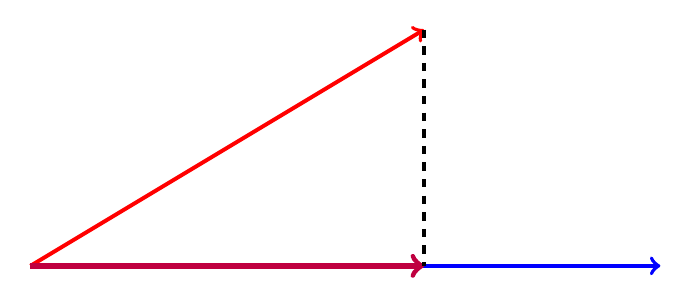
\begin{tikzpicture}
	\draw[->, color=red,line width=0.5mm](0,0)--(5,3);
	\draw[->, color=blue,line width=0.5mm](0,0)--(8,0);
	\draw[->, color=purple,line width=0.7mm](0,0)--(5,0);
	\draw[dashed, line width=0.5mm](5,3)--(5,0);
	\node[color=red] at (2.5,2) {$\vcw$};
ff	\node[color=blue] at (6.5,0.5) {$\vcv$};
	\node[color=purple] at (3,0.5) {$\proj{\vcw}{\vcv}$};
\end{tikzpicture}
\end{center}
\vspace{1em}
\end{definition}

\begin{exercise}{}
Let $$\vcv=\bmat{x\\y\\z}.$$ Show that $\proj{\vcv}{\vci}=x\cdot \vci.$ That is, show that the projection of $\vcv$ onto the unit vector in the $x$ direction is the $x$-component of $\vcv$.
\end{exercise}

\begin{exercise}{Physics in \textit{my} math?}

Suppose we have a box with mass $m$ sitting still on a slope that is $\theta$ above the horizontal.

\vspace{1em}
\begin{center}
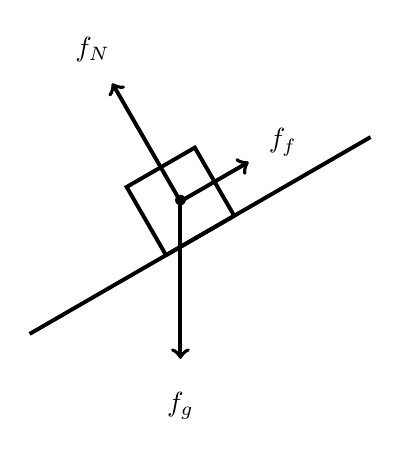
\begin{tikzpicture}
%\draw[line width=0.5mm] (-2,0)--(6.33,0);
\draw[line width=0.5mm] (0,0)--(30:5);
\draw[line width=0.5mm] (30:2)--(30:3)--(2.098,2.366)--(1.232,1.866)--(30:2);
\node at (1.915,1.683) {$\bullet$};
\draw[line width=0.5mm,->] (1.915,1.683)--(1.915,-0.317);
\node at (1.91506,-0.916987) {$f_g$};
\draw[line width=0.5mm,->] (1.915,1.683)--(1.04906,3.18297);
\node at (0.79906,3.61598) {$f_N$};
\draw[line width=0.5mm,->] (1.915,1.683)--(2.78109,2.18301);
\node at (3.2141,2.43301) {$f_f$};
\end{tikzpicture}
\end{center}
\vspace{1em}

The box is sitting still, so these three forces must be in equilibrium. That is $f_g+f_N+f_f=\vzero$.
\vspace{1em}
\begin{enumerate}
\item Explain how we know that $f_g=\bmat{0\\-mg}$.
\vspace{1em}
\item Note that $f_g$ must have a component parallel to the surface such that $f_{g\parallel}=-f_f$ and a component perpendicular to the surface such that $f_{g\perp}=-f_N$? Why?
\vspace{1em}
\item Find $f_{g\parallel}$. You can do this by taking a unit vector parallel to the slope $$\vcv_{\parallel}=\bmat{\cos\theta\\ \sin\theta}$$ then finding $f_{g\parallel}=\proj{f_g}{\vcv_\parallel}.$
\vspace{1em}
\item Find $f_{g\perp}$. You can do this by taking a unit vector perpendicular to the slope $$\vcv_{\perp}=\bmat{-\sin\theta\\ \cos\theta}$$ then finding $f_{g\perp}=\proj{f_g}{\vcv_\perp}.$
\vspace{1em}
\item Physics sez: $||f_N||=mg\cos\theta$. Do you agree?
\end{enumerate}

\end{exercise}